\documentclass[spanish,12pt,a4paper,oneside]{book}
\usepackage{newclude} % Permite usar \include* que es igual que \include pero sin saltos de página adicionales
%\includeonly{cap01} % con este comando solo se incluirán los archivos mencionados haciendo que la compilación sea mucho más rápida. Referencias a otros capítulos quedarán rotas, se recomienda una compilación limpia cada vez que se cambie esta línea (es decir, borrar ficheros intermedios cuando se descomenta/comenta/cambia el argumento)

\usepackage[textwidth=15cm, textheight=22.5cm, top=3.5cm, bottom=3.5cm,left= 4cm,right=2cm]{geometry}

\usepackage[es-tabla,es-nodecimaldot]{babel} % Cambiamos a idioma español
\usepackage[utf8]{inputenc} % Decimos que espere codificación utf-8 de los ficheros
\usepackage{csquotes} % Paquete recomendado por biblatex cuando se usa babel
\usepackage[T1]{fontenc}

\usepackage[hidelinks]{hyperref} % Referencias e índices son enlaces al contenido. La opción hidelinks hace que se vean como texto normal

\usepackage{graphicx} % Gráficos y colores
\usepackage{amsmath,amssymb}
\usepackage{float}
\usepackage{changepage}
\usepackage{subcaption}
\usepackage{url}
\usepackage[acronym]{glossaries}

\makeglossaries

\section{Glosario de términos}

\begin{tabular}{l l}
  IVI    & In Vehicle Infotainment \\
  VMM    & Virtual Machine Monitor \\
  RTOS   & Real Time Operating System \\
  IOMMU  & Input Output Memory Management Unit \\
  LCD    & Liquid Crystal Device \\
  GUI    & Graphical User Interface \\
  SoC    & System on Chip \\
  RAM    & Random Access Memory \\
  GPU    & Graphics Processing Unit \\
  eMMC   & Embedded Multi Media Card \\
  API    & Application Program Interface \\
  vCPU   & Virtual CPU \\
  vMMU   & Virtual Memory Management Unit \\
  vIRQ   & Virtual Interrupt \\
  IPC    & Inter Processor Communication \\
  DMA    & Direct Memory Access \\
  VNIC   & Virtual Network Interface Controller \\
  MIPC   & Multi-OS Inter-Process Communication \\
  VMX    & Virtual Machine Extensions \\
  HVC    & Hypervisor Call \\
  GIC    & Global Interrupt Controller \\
  AMP    & Asimetric Multiprocessing \\
  BSP    & Board Support Package \\ 
\end{tabular}



\newpage


\usepackage[table]{xcolor} % Necesaria la opción table para usar filas de colores en las tablas.

\usepackage{booktabs} % para los comandos toprule, midrule, cmidrule y bottomrule: líneas horizontales de las tablas
\usepackage{threeparttable} % Entorno para las notas a pie de tabla

%--- Paquete listings y personalizaciones ---%
\setlength{\parindent}{0em}

\setcounter{tocdepth}{3} %Numbering subsubsection and showing it in Table of Contents
\setcounter{secnumdepth}{3}

\usepackage{pdfpages}
\usepackage{pgfplots}
\usepackage{adjustbox}
\usepackage{tikz}

\usepackage{listings}
\definecolor{mGreen}{rgb}{0,0.6,0}
\definecolor{mGray}{rgb}{0.5,0.5,0.5}
\definecolor{mPurple}{rgb}{0.58,0,0.82}
\definecolor{backgroundColour}{rgb}{0.95,0.95,0.92}

\lstdefinestyle{CStyle}{
    backgroundcolor=\color{backgroundColour},
    commentstyle=\color{mGreen},
    keywordstyle=\color{magenta},
    numberstyle=\tiny\color{mGray},
    stringstyle=\color{mPurple},
    basicstyle=\footnotesize,
    breakatwhitespace=false,
    breaklines=true,
    captionpos=b,
    keepspaces=true,
    numbers=none,
    numbersep=5pt,
    showspaces=false,
    showstringspaces=false,
    showtabs=false,
    tabsize=2,
    language=C
}

\usepackage{multirow}

\usepackage{tikz}

%--- Formato de títulos ---%
\usepackage{titlesec} % Librería para cambiar el formato de \chapter, \section, ...
\titleformat{\paragraph}[runin]{\normalfont\normalsize\itshape}{\theparagraph}{1em}{} % formato de \paragraph: fuente y tamaño normales y cursiva. 1em de separación
\titleformat{\subparagraph}[runin]{\normalfont\normalsize\itshape}{\thesubparagraph}{1em}{} % formato de \subparagraph: fuente y tamaño normales y cursiva. 1em de separación

%--- AJUSTES MANUALES ---%

% Definimos un nuevo entorno para tablas con filas alternando colores:
%  - es necesario cargar el paquete xcolor con la opción table
%  - Usar los comandos \hiderowcolors y \showrowcolors cuando se quiera parar o empezar a usar la alternancia de colores dentro de una tabla
\newenvironment{stripedtable}
	{\rowcolors{2}{gray!6}{white}\begin{table}}
	{\end{table}\rowcolors{2}{}{}}

\DeclareUnicodeCharacter{FEFF}{ } %para evitar errores de compilación
%%%%%%%%%%%%%%%%%%%%%%%%%%%%% DOCUMENT %%%%%%%%%%%%%%%%%%%%%%%%%%%%%
\begin{document}

\frontmatter
%%%%%%%%%%%%%%%%%%%%%%%%%%%%% TÍTULO, RESUMEN, AGRADECIMIENTOS Y LISTAS %%%%%%%%%%%%%%%%%%%%%%%%%%%%%
%	TÍTULO
% Página con el título, hay que entrar en title.tex para modificar: nombre del trabajo, autor, tutores y fecha

%\include*{title}
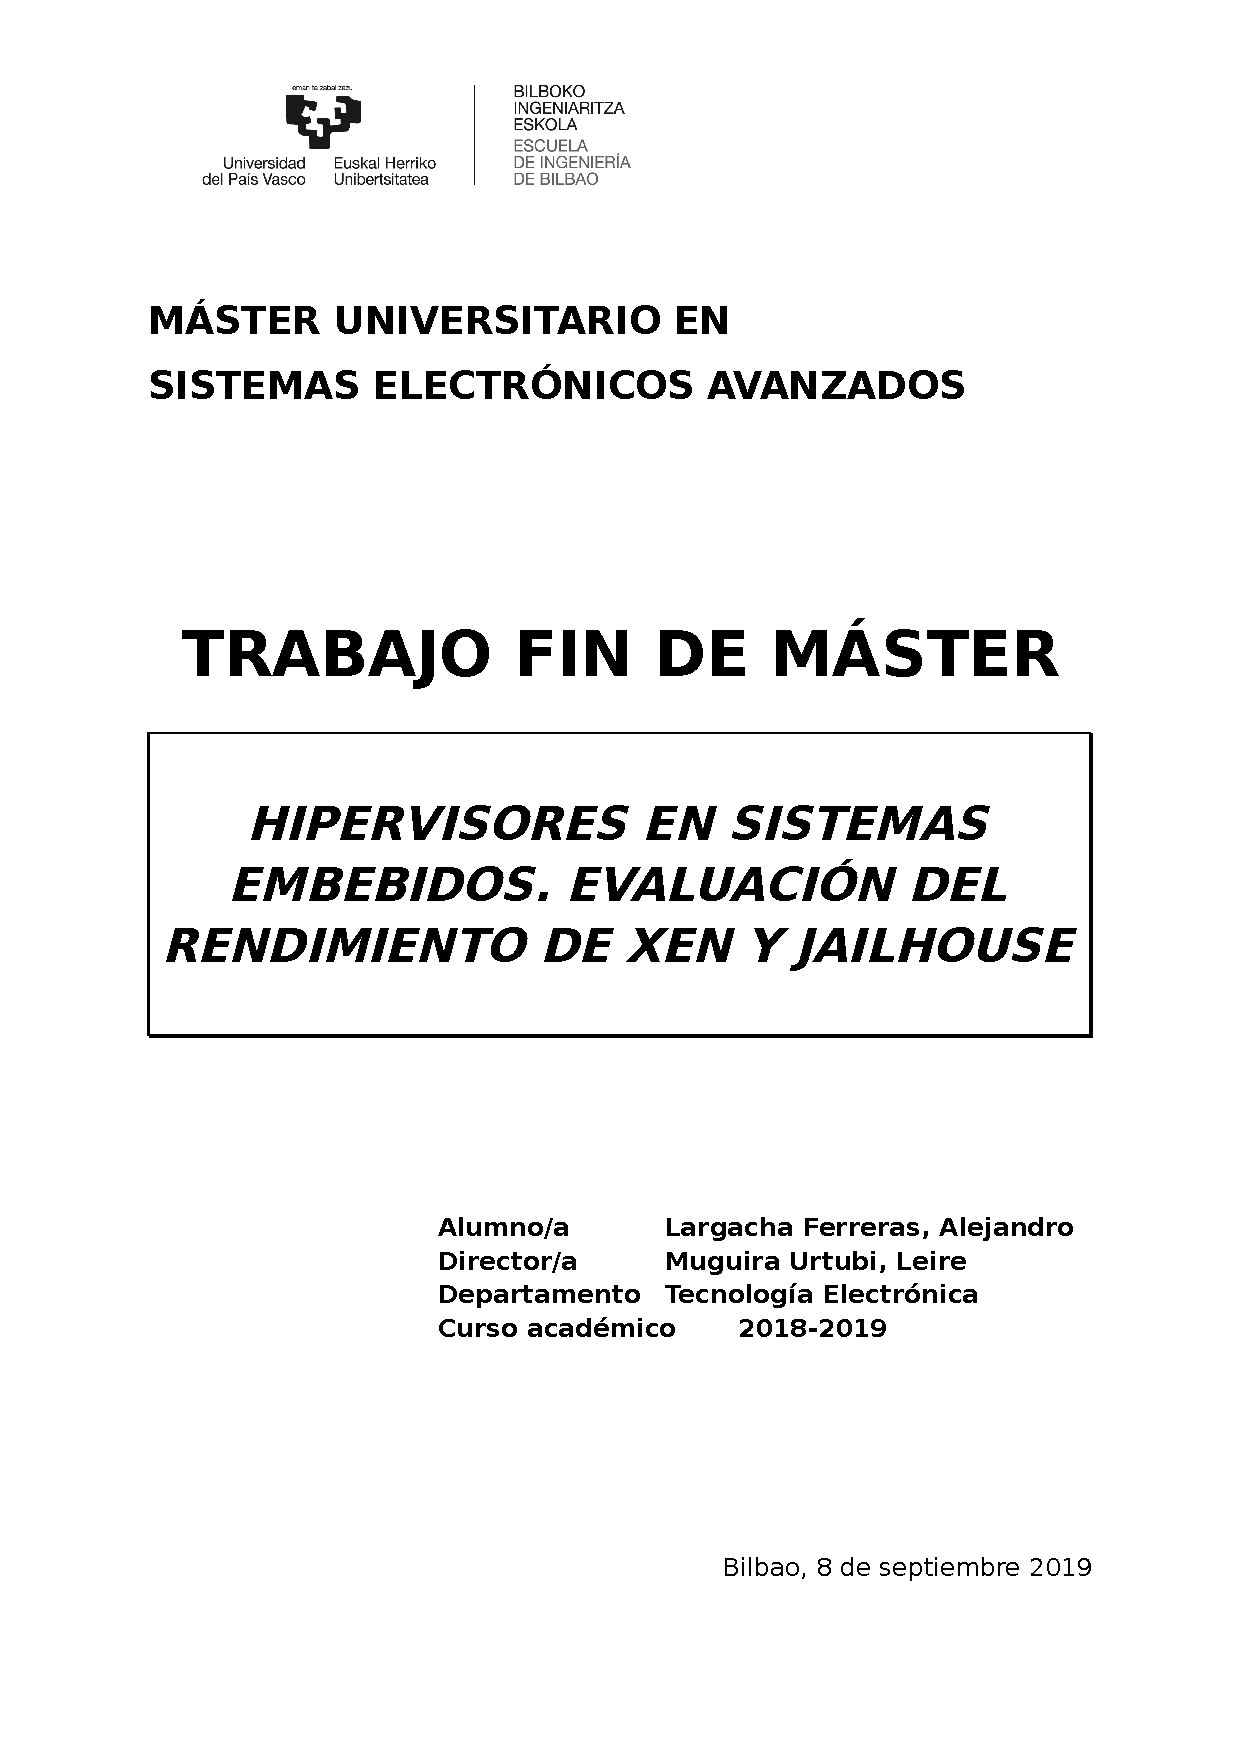
\includepdf{recursos/title.pdf}

%	ÍNDICE
\tableofcontents % indice de contenidos

%	INDICE DE FIGURAS, TABLAS Y ALGORITMOS
\listoffigures
\listoftables
\printglossary[type=\acronymtype, title={Glosario de términos}]

%%%%%%%%%%%%%%%%%%%%%%%%%%%%% CUERPO DEL TFM %%%%%%%%%%%%%%%%%%%%%%%%%%%%%
\mainmatter

\include*{cap01}

\include*{cap02}

\include*{cap03}

\include*{cap04}

\include*{cap05}

\include*{cap06}

%%%%%%%%%%%%%%%%%%%%%%%%%%%%% APÉNDICES %%%%%%%%%%%%%%%%%%%%%%%%%%%%%
\appendix
% ANEXOS
\include*{anexos}

%%%%%%%%%%%%%%%%%%%%%%%%%%%%% BACKMATTER %%%%%%%%%%%%%%%%%%%%%%%%%%%%%
\backmatter

%%% Bibliografía
\addcontentsline{toc}{chapter}{Referencias} % Para que salga en el índice general

\begin{thebibliography}{00}
	\bibitem{EmbeddedWorld2018}  Greenbaum, Jack, and Cesare Garlati. \emph{"Hypervisors in Embedded Systems. Applications and Architechtures."}. Embedded World Conference 2018.
	\bibitem{Popek1974} Popek, Gerald J., and Robert P. Goldberg. \emph{"Formal requirements for virtualizable third generation architectures."}. Communications of the ACM, Volume 17 Issue 7, July 1974.
	\bibitem{hyper_review} Mounika M., and Chinnaswamy C N. \emph{"A Comprehensive Review on Embedded Hypervisors".}. International Journal of Advanced Research in Computer Engineering \& Technology (IJARCET), Volume 5 Issue 5, May 2016.
	\bibitem{hyper_perf_arm} Toumassian, Sebouh, Werner, Rico, and Axel Sikora. \emph{"Performance Measurements for Hypervisors on Embedded ARM Processors."}. Intl. Conference on Advances in Computing, Communications and Informatics (ICACCI) , 2016.
	\bibitem{denali} Whitaker, Andrew, Shaw, Marianne, and Steven D. Gribble. \emph{"Denali: Lightweight Virtual Machines for Distributed and Networked Applications."}. The University of Washington.
  \bibitem{xvisor} Patel, Anup, Daftedar, Mai, Shalan, Mohamed, and M. Watheq El-Kharashi. \emph{"Embedded Hypervisor Xvisor: A comparative analysis."}. 23rd Euromicro International Conference on Parallel, Distributed, and Network-Based Processing, 2015.
  \bibitem{vmware} \url{https://www.vmware.com/products/esxi-and-esx.html}
  \bibitem{jailhouse_github} \url{https://github.com/siemens/jailhouse}
  \bibitem{okl4} Heiser, Gernot, and Ben Leslie, \emph{"The OKL4 Microvisor: Convergence Point of Microkernels and Hypervisors."}. Proceedings of the 1st ACM SIGCOMM Asia-Pacific Workshop on Systems, ApSys 2010, New Delhi, India, 2010.
  \bibitem{hyper-v} \url{https://docs.microsoft.com/es-es/virtualization/hyper-v-on-windows/about/}
  \bibitem{seL4} \url{https://sel4.systems/}
  \bibitem{okl4_2} \url{https://gdmissionsystems.com/-/media/General-Dynamics/Cyber-and-Electronic-Warfare-Systems/PDF/Data-Sheets/okl4-hypervisor-datasheet.ashx?la=en}
  \bibitem{windriver_1} WindRiver Hypervisor Product Note \url{https://www.windriver.com/products/product-notes/wind-river-hypervisor-product-note.pdf}


  \bibitem{kvm_1} Dall, Christoffer, Li, Shih-Wei, Lim, Jin Tack, Nieh, Jason, and Georgios Koloventzos. \emph{"Arm Virtualization: Performance and Architectural Implications."}. ACM/IEEE 43rd Annual International Symposium on Computer Architecture, 2016.
	\bibitem{kvm_2} \url{https://lwn.net/Articles/705160/}
  \bibitem{kvm_list} \url{https://www.linux-kvm.org/page/Guest_Support_Status}
  \bibitem{xen_arm_whitepaper} \url{https://wiki.xenproject.org/wiki/Xen_ARM_with_Virtualization_Extensions_whitepaper}
  \bibitem{jailhouse_p1} Valentine Sinitsyn. \emph{"Understanding the Jailhouse hypervisor, part 1"} \url{https://lwn.net/Articles/578295/}
  \bibitem{jailhouse_p2} Valentine Sinitsyn.\emph{"Understanding the Jailhouse hypervisor, part 2"} \url{https://lwn.net/Articles/578852/}
  \bibitem{jailhouse_elc2017} Ramsauer, Ralf, Kiszka, Jan, and Wolfgang Mauerer. \emph{"Building Mixed Criticality Linux Systems with the Jailhouse Hypervisor"} \url{https://elinux.org/images/4/45/ELC17-Ramsauer-Kiszka.pdf}. Embedded Linux Conference 2017.
  \bibitem{jailhouse_isolation} Danielsson, Jakob, Seceleanu, Tiberiu, Jagemar, Marcus, Behnam, Moris, and Mikael Sjodin. \emph{"Testing Performance-Isolation in Multi-Core Systems."}. IEEE 43rd Annual Computer Software and Applications Conference (COMPSAC), 2019.



  \bibitem{avnet_github} \url{https://github.com/Avnet/bdf}
  \bibitem{saleae} \url{https://eur.saleae.com/products/saleae-logic-8}
  \bibitem{jtag_hs2} \url{https://www.digikey.es/es/product-highlight/d/digilent/jtag-hs2-programming-cable}
  \bibitem{vivado_suite_2018_3} \url{https://www.xilinx.com/products/design-tools/vivado.html}
  \bibitem{xsdk_suite_2018_3}\url{https://www.xilinx.com/products/design-tools/embedded-software/sdk.html}
  \bibitem{yocto_project_url}\url{https://www.yoctoproject.org/}
  \bibitem{petalinux_suite_2018_3}\url{https://www.xilinx.com/products/design-tools/embedded-software/petalinux-sdk.html}

  \bibitem{ultra96_url} \url{https://www.96boards.org/product/ultra96/}

	\bibitem{armv8_el} \url{https://developer.arm.com/docs/100878/latest/changing-exception-levels}
%Xilinx stuff
  \bibitem{axi_gpio} AXI GPIO v2.0 LogiCORE IP Product Guide. \url{https://www.xilinx.com/support/documentation/ip_documentation/axi_gpio/v2_0/pg144-axi-gpio.pdf}
  \bibitem{axi_trm} Zynq UltraScale+ Device Technical Reference Manual \url{https://www.xilinx.com/support/documentation/user_guides/ug1085-zynq-ultrascale-trm.pdf}
  \bibitem{axi_timer} AXI Timer v2.0 LogiCORE IP Product Guide. \url{https://www.xilinx.com/support/documentation/ip_documentation/axi_timer/v2_0/pg079-axi-timer.pdf}
  \bibitem{mpsoc_registers} Zynq UltraScale+ Devices Register Reference. \url{https://www.xilinx.com/html_docs/registers/ug1087/ug1087-zynq-ultrascale-registers.html}
  \bibitem{xen_source} \url{http://xenbits.xen.org/gitweb/?p=xen.git}
  \bibitem{xen_source_xilinx} \url{https://github.com/Xilinx/xen}
  \bibitem{armv8_stage2} \url{https://developer.arm.com/architectures/learn-the-architecture/armv8-a-virtualization/stage-2-translation}
  \bibitem{xen_domU_xsdk} \url{https://xilinx-wiki.atlassian.net/wiki/spaces/A/pages/18842536/XEN+EL1+Baremetal+DomU}
\end{thebibliography}

\end{document}
